\documentclass[11pt,a4paper,titlepage]{article}
\usepackage[utf8]{inputenc}
\usepackage[english]{babel}
\usepackage[T1]{fontenc}

\RequirePackage[layout=inline]{fixme}

\usepackage{float}
\usepackage{graphicx}
\usepackage{setspace}
\usepackage{amsmath}
\usepackage{courier}
\usepackage{amsmath}
\usepackage{listings}
\usepackage{color}
\usepackage[toc, page]{appendix}

\usepackage{algpseudocode}
\usepackage[bottom]{footmisc}
\usepackage{verbatimbox}

\usepackage{changepage}

\definecolor{mygreen}{rgb}{0,0.6,0}
\definecolor{mygray}{rgb}{0.5,0.5,0.5}
\definecolor{mymauve}{rgb}{0.58,0,0.82}




\lstset{ %
	backgroundcolor=\color{white},   % choose the background color
	basicstyle=\scriptsize,        % size of fonts used for the code
	breaklines=true,                 % automatic line breaking only at whitespace
	captionpos=b,                    % sets the caption-position to bottom
	commentstyle=\color{mygreen},    % comment style
	escapeinside={\%*}{*)},          % if you want to add LaTeX within your code
	keywordstyle=\color{blue},       % keyword style
	stringstyle=\color{mymauve},     % string literal style
	numbers=left,
}

%\renewcommand{\thesubsection}{\thesection.\alph{subsection}}



\usepackage{booktabs}
\usepackage[backend=biber, bibencoding=utf8, style=ieee]{biblatex}

\addbibresource{references.bib}
\usepackage[final,hidelinks]{hyperref} % must be last package loaded

\author{Ólafur Jón Thoroddsen}  % My name, for the titlepage
\title{\includegraphics{graphics/ru-logo}\\\vspace{10mm}
	Mechatronics II\\T-535-MECH \ \\Homework 6}  % The title, for the titlepage

\begin{document}
	\pagenumbering{arabic}
	\maketitle
	
	\tableofcontents
	\pagebreak
	
	\section{Sending variable values over USART\label{sec:usarthex}}
	
	When data is sent over USART to a terminal screen, it is interpreted by the terminal as ASCII~\cite{ascii} code. The mapping from values to symbols is shown in figure~\ref{fig:ascii}, as an example, the value $53_{\text{D}}$ = 0x35 is mapped to the character '5'. Note that there is a huge difference between the character '5' and the number 5. The first 32 entries in the ASCII table are special symbols that can sometimes perform actions, e.g. the symbol at index $10_{\text{D}}$ = 0x0A is a newline character.
	
	\begin{figure}[h]
		\centering
		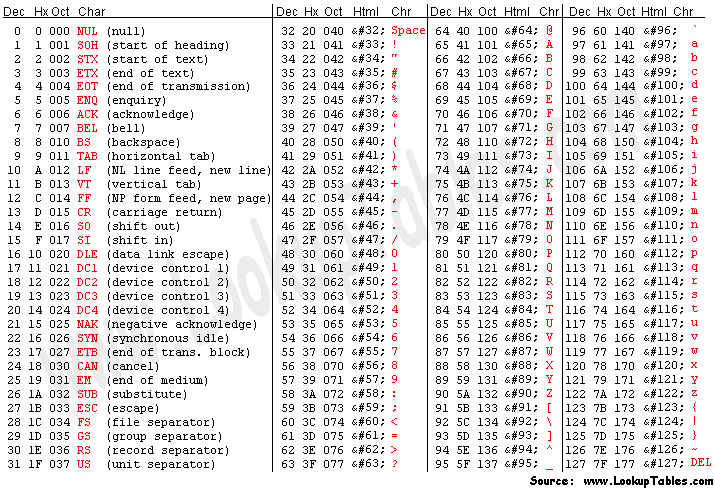
\includegraphics[width=\textwidth]{graphics/ascii}
		\caption{The 7-bit ASCII table.}
		\label{fig:ascii}
	\end{figure}
	
	\subsection{Writing bytes (8 bits) as Hexadecimals}
	
	A single byte is 8 bits. Conveniently, all single symbol hex numbers (0x0 - 0xF) are representable by 4 bits. Thus, with only two hex numbers we can represent the entire 8 bits. The tricky part is mapping from values to the indexes of the characters representing that value in the ASCII table.
	
	Using the fact that 4 bits are completely representable by a single hex number we split our 8 bit number into two halves, storing the lower 4 bits (least significant nibble) and upper 4 bits (most significant nibble) separately, yielding two 8 bit numbers as shown in figure~\ref{fig:nibbleshift}
	\begin{figure}[h]
		\centering
		\fbox{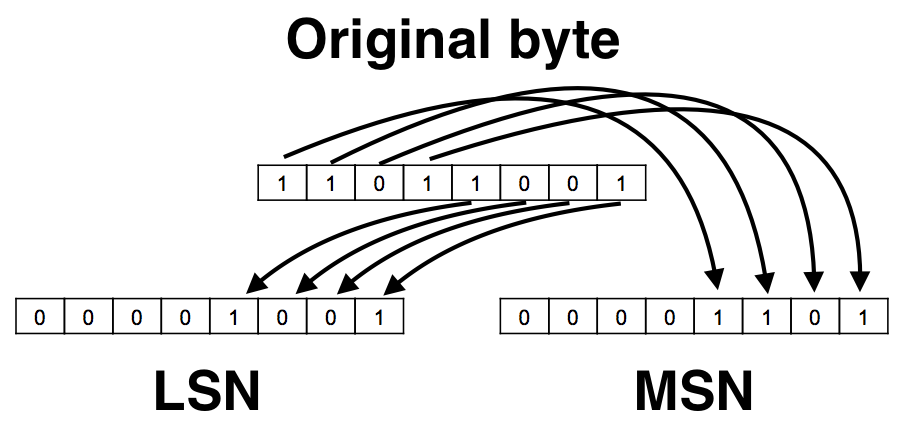
\includegraphics[width=0.8\textwidth]{graphics/nibbleshift}}
		\caption{Shifting and masking the original byte into two separate bytes, each with a value in the range 0x00 - 0x0F}
		\label{fig:nibbleshift}
	\end{figure}
	
	\pagebreak
	\noindent In code this is implemented as shown here below.
	
	\vspace{5mm}
	\lstinputlisting[language=c,frame=single,firstline=80,lastline=82,firstnumber=80]{../usart_advanced/myUSART.c}\vspace{5mm}
	
	\noindent Now, to map from the value to the corresponding index in the ASCII table, there are two cases to consider. If we have a digit (0-9) or a letter (A-F). This is necessary because these symbols are not in succession in the ASCII table.
	\begin{enumerate}
		\item[Case 1] In the ASCII table (fig.~\ref{fig:ascii}) we can see that the index of the symbol '0' is 0x30. Thus, to map from digits to their symbol indexes, we simply add 0x30 to their value.
		\item[Case 2] Now, if we do not have a digit, then we must have a letter in [A,F]. Looking at the ASCII table, we compute the difference between the index of the symbol 'A' and 0x0A, which yields 0x37.
	\end{enumerate}
	
	\noindent In code, I implemented this as a macro function.
	
	\vspace{5mm}
	\lstinputlisting[language=c,frame=single,firstline=11,lastline=14,firstnumber=11]{../usart_advanced/myUSART.c}
	
	\noindent Now we can simply transmit the MSN and LSN directly using our\\\verb|USART_Transmit()| function (see Appendix~\ref{sec:usartappendix}). I add the '0x' in front of MSN and LSN to indicate in erminal screen that this is a hex value. Transmitting 0x0A results in a new line after second digit.
	\lstinputlisting[language=c,frame=single,firstline=87,lastline=91,firstnumber=87]{../usart_advanced/myUSART.c}
	The entire function can be seen in Appendix~\ref{sec:usartappendix}

	The function can be tested by simply declaring an 8 bit variable and use it as an argument to the function as seen in figure~\ref{fig:8bitsend}.
	
	\begin{verbbox}
		USART_Transmit_8_hex()
	\end{verbbox}
	\begin{figure}[h]
		\centering
		\fbox{\includegraphics[width=\textwidth]{graphics/8bitsend}}
		\caption{Testing the function \theverbbox using an arbitrary 8 bit hex value}
		\label{fig:8bitsend}
	\end{figure}
	
	\subsection{Writing ints (16 bits) as Hexadecimals}
		To write a 16 bit value in hex on rminal screen, we follow exactly the same procedure as we did for 8 bits, except we need 4 symbols this time, so we shift and mask two more times.
		\lstinputlisting[language=c,frame=single,firstline=57,lastline=61,firstnumber=57]{../usart_advanced/myUSART.c}
		
		\noindent Now that we have split our 16 bit number into four nibbles, we convert each nibble as we did for the 8 bits and then transmit one character at a time over USART.
		
		\lstinputlisting[language=c,frame=single,firstline=63,lastline=75,firstnumber=63]{../usart_advanced/myUSART.c}
		
		\noindent Testing the module is performed by sending a 16 bit number to terminal using the function as seen in figure~\ref{fig:16bitsend}.
		
		\begin{verbbox}
			USART_Transmit_16_hex()
		\end{verbbox}
		\begin{figure}[h]
			\centering
			\fbox{\includegraphics[width=\textwidth]{graphics/16bitsend}}
			\caption{Testing the function \theverbbox using an arbitrary 16 bit hex value}
			\label{fig:16bitsend}
		\end{figure}
		
		\subsection{Writing long (32 bits) as Hexadecimals}
		
		Writing 32 bit variables to the terminal screen in hex format is again just more repetitions of the same actions as before. In the implementation of this function I took a more compact approach using loops and pointers to reference to the places in memory where my intermediate variables are stored. The entire function can be seen here below.
		
		\lstinputlisting[language=c,frame=single,firstline=42,lastline=54,firstnumber=42]{../usart_advanced/myUSART.c}
		
		\noindent The effect of this function is exactly the same as for the 16 and 8 bit versions, except that this one creates more intermediate variables. This could possibly be optimized even further by reducing the function to a single for loop instead of two. The test case is done similar to before as seen in figure~\ref{fig:32bitsend}
		
		\begin{verbbox}
			USART_Transmit_32_hex()
		\end{verbbox}
		\begin{figure}[h]
			\centering
			\fbox{\includegraphics[width=\textwidth]{graphics/32bitsend}}
			\caption{Testing the function \theverbbox using an arbitrary 32 bit hex value.}
			\label{fig:32bitsend}
		\end{figure}


	
	\pagebreak
	\section{Formatting for decimal}
	Viewing the values of variables in decimal format is trickier then the hexadecimal format because we cannot split the bit pattern up into discrete parts like we did for the hexadecimal representation. The main ideas behind the following (8 bit) algorithm is integer division and modulo arithmetic.
	\vspace{3mm}
			\begin{algorithmic}
				\If {$byte < 10$}
					\State \verb|USART_Transmit|(byte)
				\ElsIf {$byte < 100$}
					\State MSN = byte / 10 // Most significant number
					\State LSN = byte \% 10 //  Least significant number
					\State MSN += 48	// Offset for the ASCII table
					\State LSN += 48	// Offset for the ASCII table
					\State \verb|USART_Transmit|(MSN)
					\State \verb|USART_Transmit|(LSN)
				\ElsIf{$byte \ge 100$}
					\State MSN = byte / 100
					\State \text{$LSN_1$} = (byte - (byte/100)*100) / 10
					\State \text{$LSN_2$} = (byte - (byte/100)*100) \% 10
					\State MSN += 48
					\State \text{$LSN_2$} + 48
					\State \text{$LSN_1$} + 48
					\State \verb|USART_Transmit|(MSN)
					\State \verb|USART_Transmit|(\text{$LSN_2$})
					\State \verb|USART_Transmit|(\text{$LSN_1$})
				\EndIf
			\end{algorithmic}

	
	\section{Printing strings\label{sec:usartstrings}}
	Strings in \verb|C| are just an array of character variables. To implement a printing function, I simply used the \verb|USART_Transmit()| function, no conversion is required this time because I'm assuming the input to this function is a character array.
	
	The input to the function is a character array and it's length. The function then sends the characters one by one to the terminal screen using USART until it comes to the defined length of the array or it reaches the NULL character '\textbackslash0'. The \verb|C| implementation and a test case can be seen below and in figure~\ref{fig:stringsend}.
	
	\pagebreak
	\lstinputlisting[language=c,frame=single,firstline=112,lastline=120,firstnumber=112]{../usart_advanced/myUSART.c}
	
	
	\begin{verbbox}
		myPrint()
	\end{verbbox}
	\begin{figure}[h]
		\centering
		\fbox{\includegraphics[width=\textwidth]{graphics/stringsend}}
		\caption{Testing the \theverbbox function}
		\label{fig:stringsend}
	\end{figure}
	
	
	\pagebreak
	\section{Progress with my project}
	
	\subsection{Last week}
	This week I worked on the SPI communication interface to the IMU sensor. It proved to be a bit of a challenge and there are still some kinks to weed out. I am unsure of how to interpret the results of my initial testing, I got a response from the sensor but when it stood still on the table the readout from was 0xFFFF. This is something I will look better into during this coming week.
	
	I built my first prototype using some wood I had laying around in the lab, screwed the motors on it and stuck a mini breadboard on there to test things out. This will provide a testing platform for the IMU sensor and motor control.
	
	I now have a much more comprehensive debug module that I described in~\ref{sec:usarthex} -~\ref{sec:usartstrings}. It will be an essential part of testing, especially the IMU communications module.
	
	
	\subsection{Next week}
	
	\begin{table}[h]
		\centering
		\begin{tabular}{llc}
			\toprule
			Task no.	&	Task	&	ETC\footnotemark\\
			\midrule
			1	&	\begin{tabular}{@{}l@{}}Debug the IMU sensor readout\\\end{tabular} &	5 hours \\	
			\midrule	
			2	&	\begin{tabular}{@{}l@{}}Find out if the PWM\\ functionalities in ATmega are\\worth replacing my own with.\end{tabular}	&	2 hours\\
			\midrule
			3	&	\begin{tabular}{@{}l@{}}If worth pursuing further, write a \\PWM module using the ATmega\\built in functionalities\end{tabular}	&	10 hours\\
			\midrule
			4	&	\begin{tabular}{@{}l@{}}Test the accuracy of the\\IMU sensor\end{tabular}	&	5 hours\\
			\midrule
			5	&		\begin{tabular}{@{}l@{}}Plan the control system and\\start designing at a high level\end{tabular}	&	5 hours\\
			\bottomrule
		\end{tabular}
		\label{tab:nextweek}
	\end{table}
	
	
	\footnotetext{Estimated Time to Complete}
	\pagebreak
	\subsection{Long term plan}
	
	\begin{table}[h]
		\centering
		\hspace*{-2cm}
		\begin{tabular}{lccc}
			\toprule
			Week	&	Software design	&	Mechanical design	&	Testing\\
			\midrule
			7	&	PID, PWM	&	Robot chassis	&	IMU \& PWM\\
			\midrule
			8	&	Rethink IMU \& PWM	&	\begin{tabular}{@{}l@{}}Power circuitry\\2nd prototype\end{tabular}	&	\begin{tabular}{@{}l@{}}Estimate power consumption\\PID motor control\end{tabular}\\
			\midrule
			9	&	Rethink PID control	&	3D drawing of the robot	&	Power consumption	\\
			\midrule
			10	&	\begin{tabular}{@{}l@{}}Integrate IMU, PID\\ and PWM modules\end{tabular}	&	Altium schematics of electronics	&	Integration\\
			\midrule
			11	&	Integration	&	Integration	&	Integration	\\
			\midrule
			12	&	Everything	&	Report layout design	&	Integration	\\
			\bottomrule
		\end{tabular}
		\label{tab:longterm}
		\hspace*{-2cm}
	\end{table}
	
	
\pagebreak
\section*{Appendices}
\appendix
\section{myUSART.c\label{sec:usartappendix}}
\lstinputlisting[language=c,frame=single]{../usart_advanced/myUSART.c}


\pagebreak
\printbibliography

\end{document}